\begin{figure}[p]
  \centering\begin{tikzpicture}
\node[inner sep=0pt] (img1) at (-0.025\textwidth, 0.00\textwidth)
    {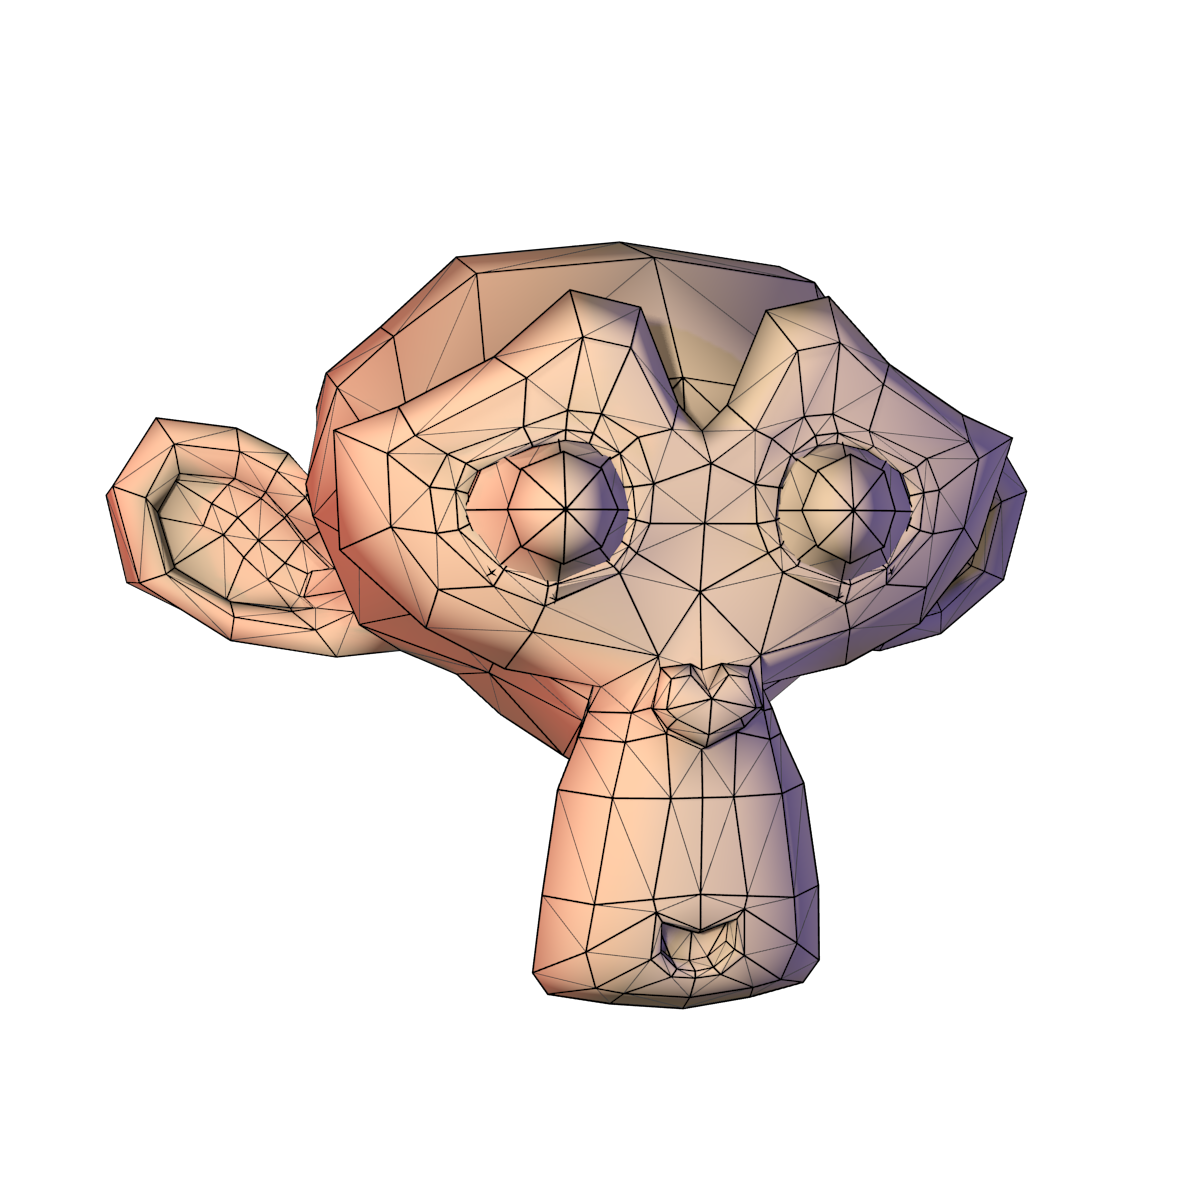
\includegraphics[width=0.25\textwidth]{./img/raw/coord-ruimtes/model_ruimte.png}};
    
\node[inner sep=0pt] (img1) at (0.0\textwidth, -0.425\textwidth)
    {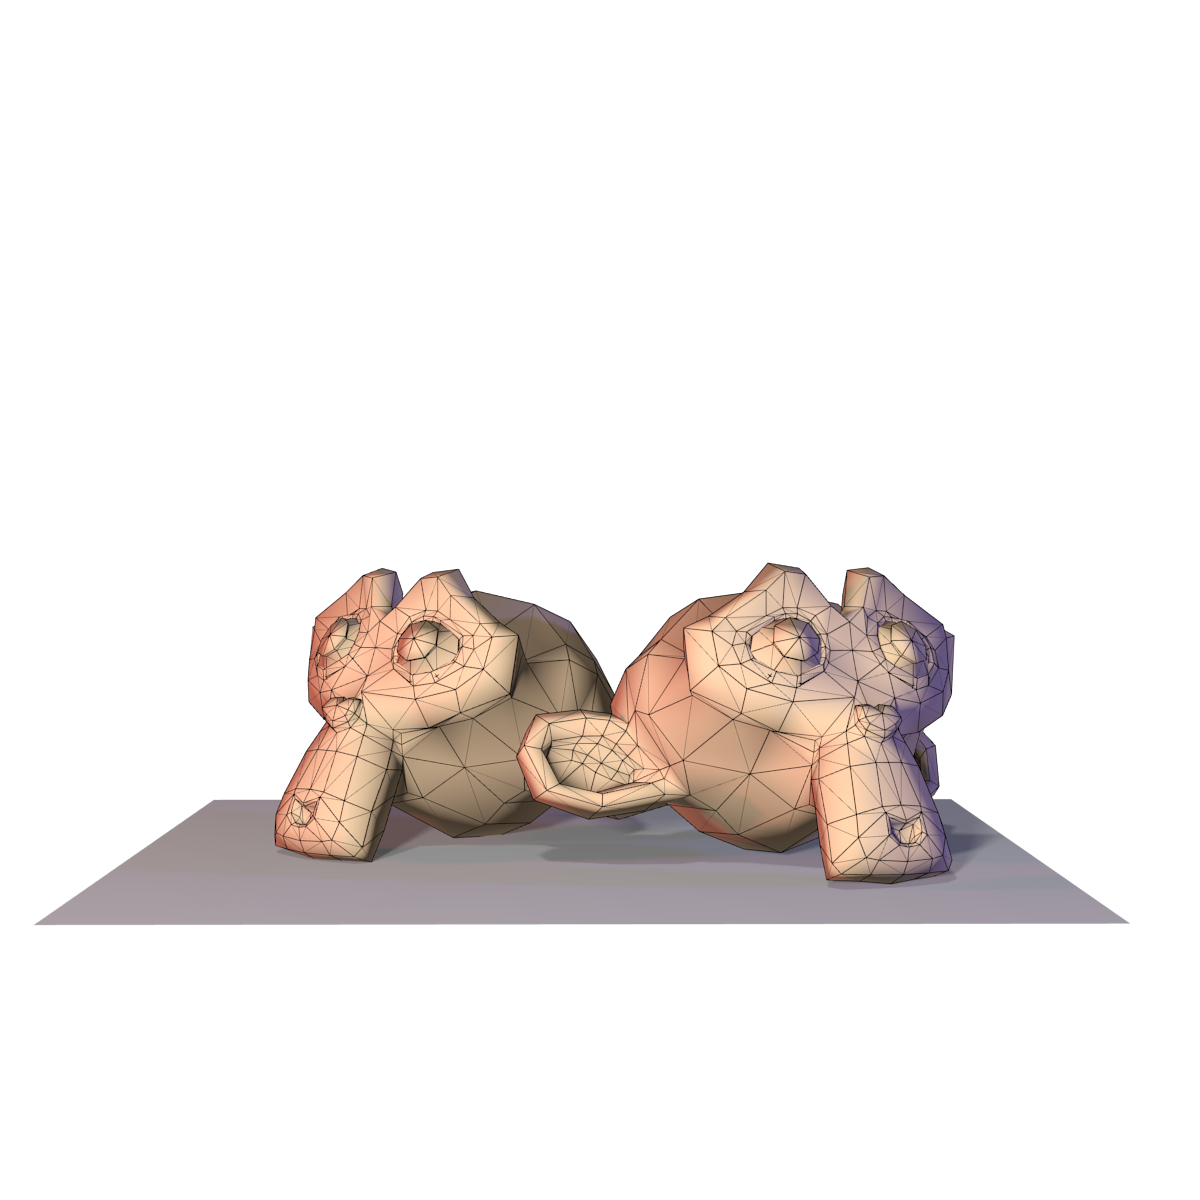
\includegraphics[width=0.6\textwidth]{./img/raw/coord-ruimtes/wereld_ruimte.png}};
\node[inner sep=0pt] (img1) at (0.0\textwidth, -0.425\textwidth)
    {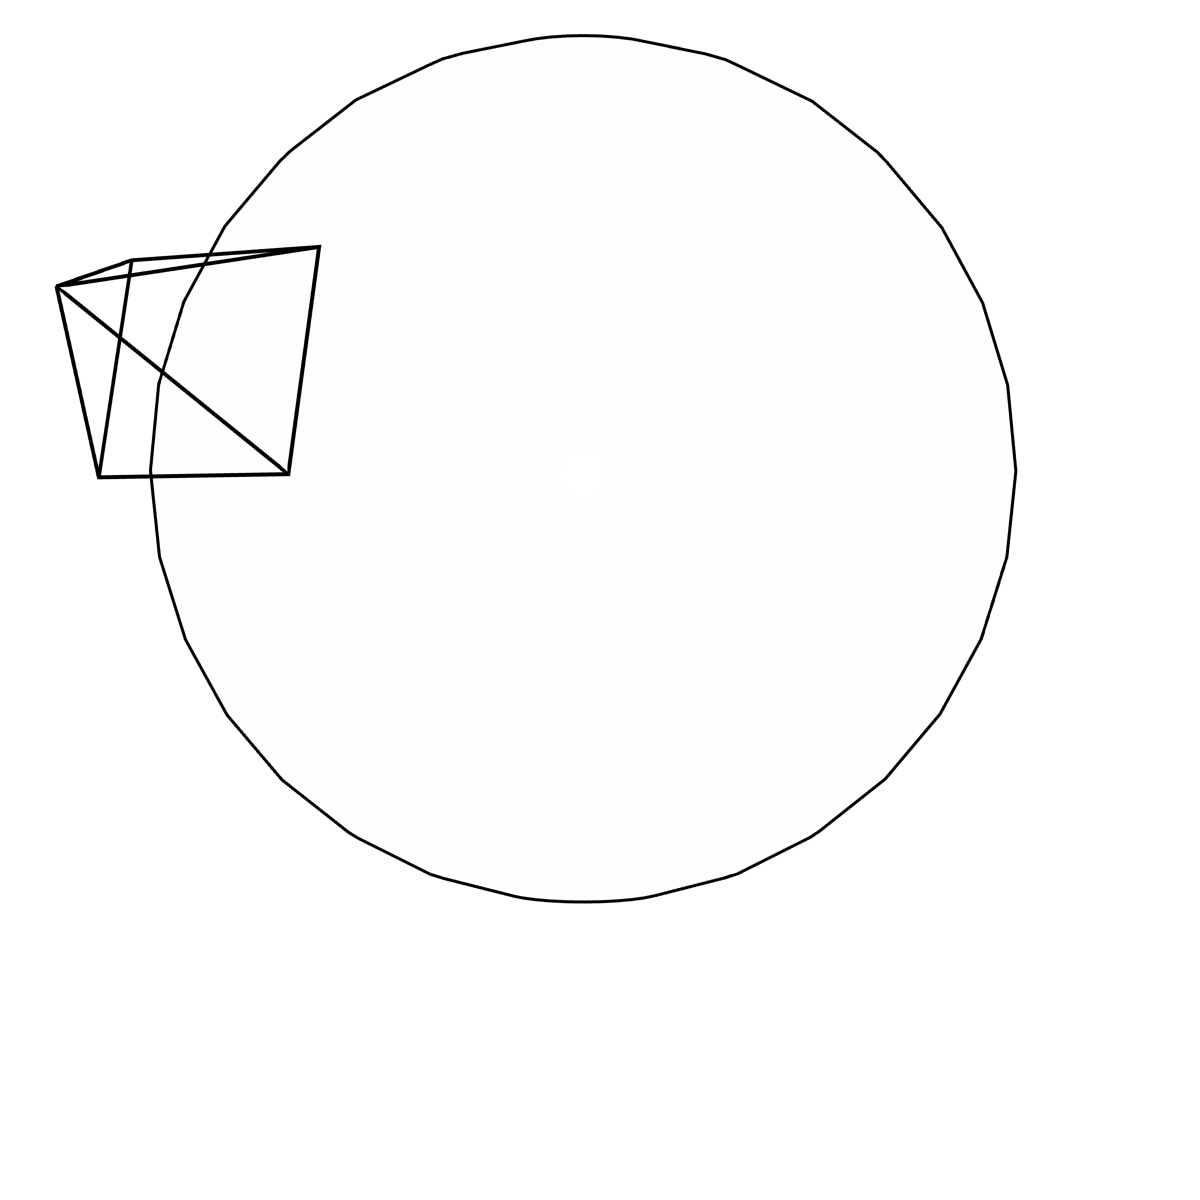
\includegraphics[width=0.6\textwidth]{./img/raw/coord-ruimtes/wereld_ruimte2.png}};
    
\node[inner sep=0pt] (img1) at (0.0\textwidth, -0.915\textwidth)
    {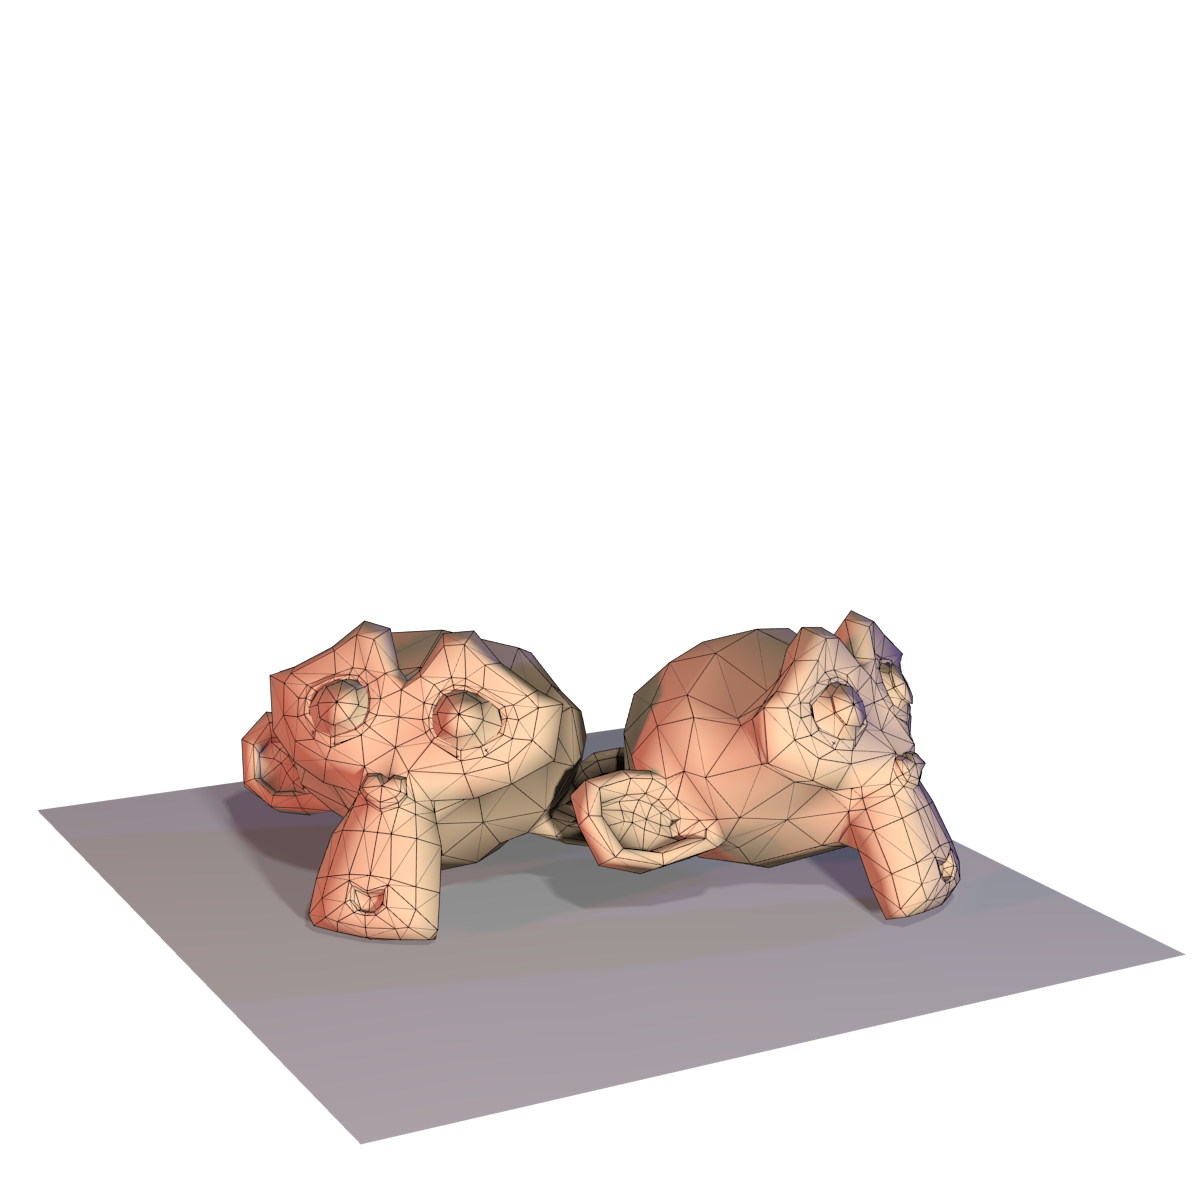
\includegraphics[width=0.6\textwidth]{./img/raw/coord-ruimtes/camera_ruimte.png}};
\node[inner sep=0pt] (img1) at (0.0\textwidth, -0.915\textwidth)
    {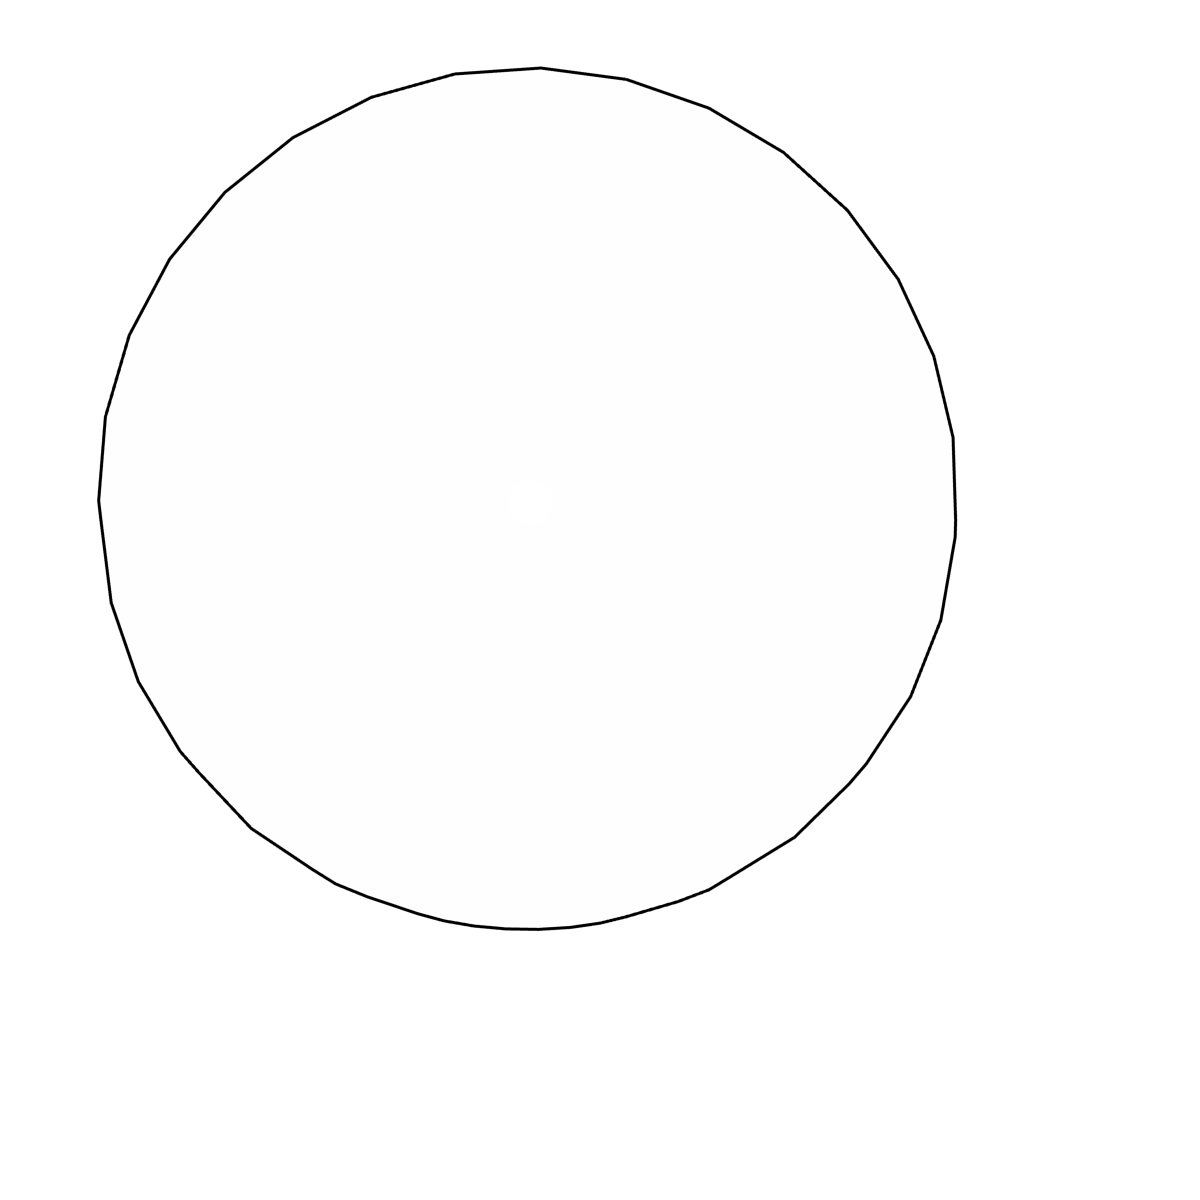
\includegraphics[width=0.6\textwidth]{./img/raw/coord-ruimtes/camera_ruimte2.png}};

\draw[-stealth, thick] (-0.005\textwidth,-0.1\textwidth) -- (-0.005\textwidth,-0.135\textwidth);
\draw[stealth-, thick] (-0.015\textwidth,-0.1\textwidth) -- (-0.015\textwidth,-0.135\textwidth);

\draw[-stealth, thick] (-0.005\textwidth,-0.6\textwidth) -- (-0.005\textwidth,-0.635\textwidth);
\draw[stealth-, thick] (-0.015\textwidth,-0.6\textwidth) -- (-0.015\textwidth,-0.635\textwidth);

\node (l3) at (0.2\textwidth, -0.1175\textwidth) {Object transformatiematrix};
\node (l3) at (0.2\textwidth, -0.6175\textwidth) {LookAt camera matrix};
\end{tikzpicture}
  \caption{Verschillende Carthesische co\"ordinatenstelsels en bijbehorende transformaties.}
  \label{fig:coord-ruimtes}
\end{figure}
